\section{Method}
The coulomb interaction for a system of ionic charges with periodicity is:
\begin{flalign}
    (4\pi\epsilon_o)U &= \frac{1}{2}\sum_{\vec{M}= -\infty}^{\infty}{' \sum_{j=1}^{n_p}\sum_{k=1}^{n_p} \frac{q_jq_k}{|\vec{r_j}-\vec{r_k}+\vec{M}.\vec{L}|}} \label{eq:main}
\end{flalign}
Here $\vec{M} \in \mathbb{Z}^2$ or $\mathbb{Z}^3 $ for a 2D or 3D periodic system respectively.  \newline
The ewald method splits the summation into two parts as:
\begin{flalign*}
    \frac{1}{r} = \frac{erf(\alpha r)}{r} + \frac{erfc(\alpha r)}{r}
\end{flalign*}
Here $\alpha$ is the ewald splitting parameter. \newline
The expression for real space summation is same in both the cases with different minimum image conventions as:
\begin{flalign*}
    (4\pi\epsilon_o)U^{SR} & = \frac{1}{2}\sum_{j=1}^{n_p}\sum_{k=1}^{n_p} \, q_j q_k \frac{erfc(\alpha|\vec{r_j}-\vec{r_k}|)}{|\vec{r_j}-\vec{r_k}|} \,
\end{flalign*}
Given the rapid decay of the function $erfc(r)/r$ as $r$ increases, the interactions with periodic images outside the box become less significant, allowing us to omit the $\vec{M}.\vec{L}$ terms. \\
The reciprocal space summation would be written as:
\begin{flalign*}
    (4\pi\epsilon_o)U^{LR} & = \frac{1}{2}\sum_{\vec{M}=-\infty}^{\infty}\prime\sum_{j=1}^{n_p}\sum_{k=1}^{n_p}\, q_j q_k \frac{erf(\alpha|\vec{r_j}-\vec{r_k}+\vec{M}.\vec{L}|)}{|\vec{r_j}-\vec{r_k}+\vec{M}.\vec{L}|} \,
\end{flalign*}
The main difference between 3d and 2d periodic case arise when we transform this summation in the reciprocal (fourier) space. Since we don't have a summation over $m_z$, which accounts for the periodicity in the Z direction, this absence breaks the symmetry in the summation and the following different expression is obtained for 2d ewald:
\begin{flalign*} 
    (4\pi\epsilon_o)U_I^{LR}& = \frac{1}{L_xL_y}\sum_{{K}=-\infty}^{\infty} \prime \int_{-\infty}^{\infty} du \frac{{exp}\left(-\frac{\sigma^2+\psi^2 +u^2}{4\alpha^2}\right)}{\sigma^2+\psi^2 +u^2}\,|S(\vec{K},u)|^2 + \\ & \quad\quad\quad\quad\quad \frac{2\sqrt{\pi}}{L_xL_y} \sum_{j=1}^{n_p}\sum_{k=1}^{n_p}q_j q_k
    \left[\frac{1-exp(-z_{jk}^2\alpha^2)}{\alpha}+\sqrt{\pi}z_{jk}\,{erf}(\alpha z_{jk})\right] \\
    S(\vec{K},u)&=\sum_{j=1}^{n_p}q_j\,exp[i(\sigma(k_x)x_{j} + \psi(k_y)y_{j}+uz_{j})]
\end{flalign*}
The above formulation was given by \colorbox{yellow}{kawata et al.}. We have an integral over $k_z$ because there's no periodicity in the $z$-direction, so the summation over $k_z$ becomes a continuous Fourier transform instead of a discrete sum.
\section{Improvement \colorbox{yellow}{(maybe a fancy name)}}
\subsection{Top-hat function}
A vacuum is introduced within our unit cell along the $z$-axis, resulting in a total length of $L_{z}$ in this direction. It is crucial that $L_{z}$ is no less than twice the original side length $L$ of the box. This requirement prevents atoms from adjacent periodic images from intruding into the non-zero zone of $\phi(z)$, which could otherwise lead to unwanted periodic effects along the $z$-axis.
\begin{figure}[H]% if you want to fix the position of this image, add H inside the []
    \centering
    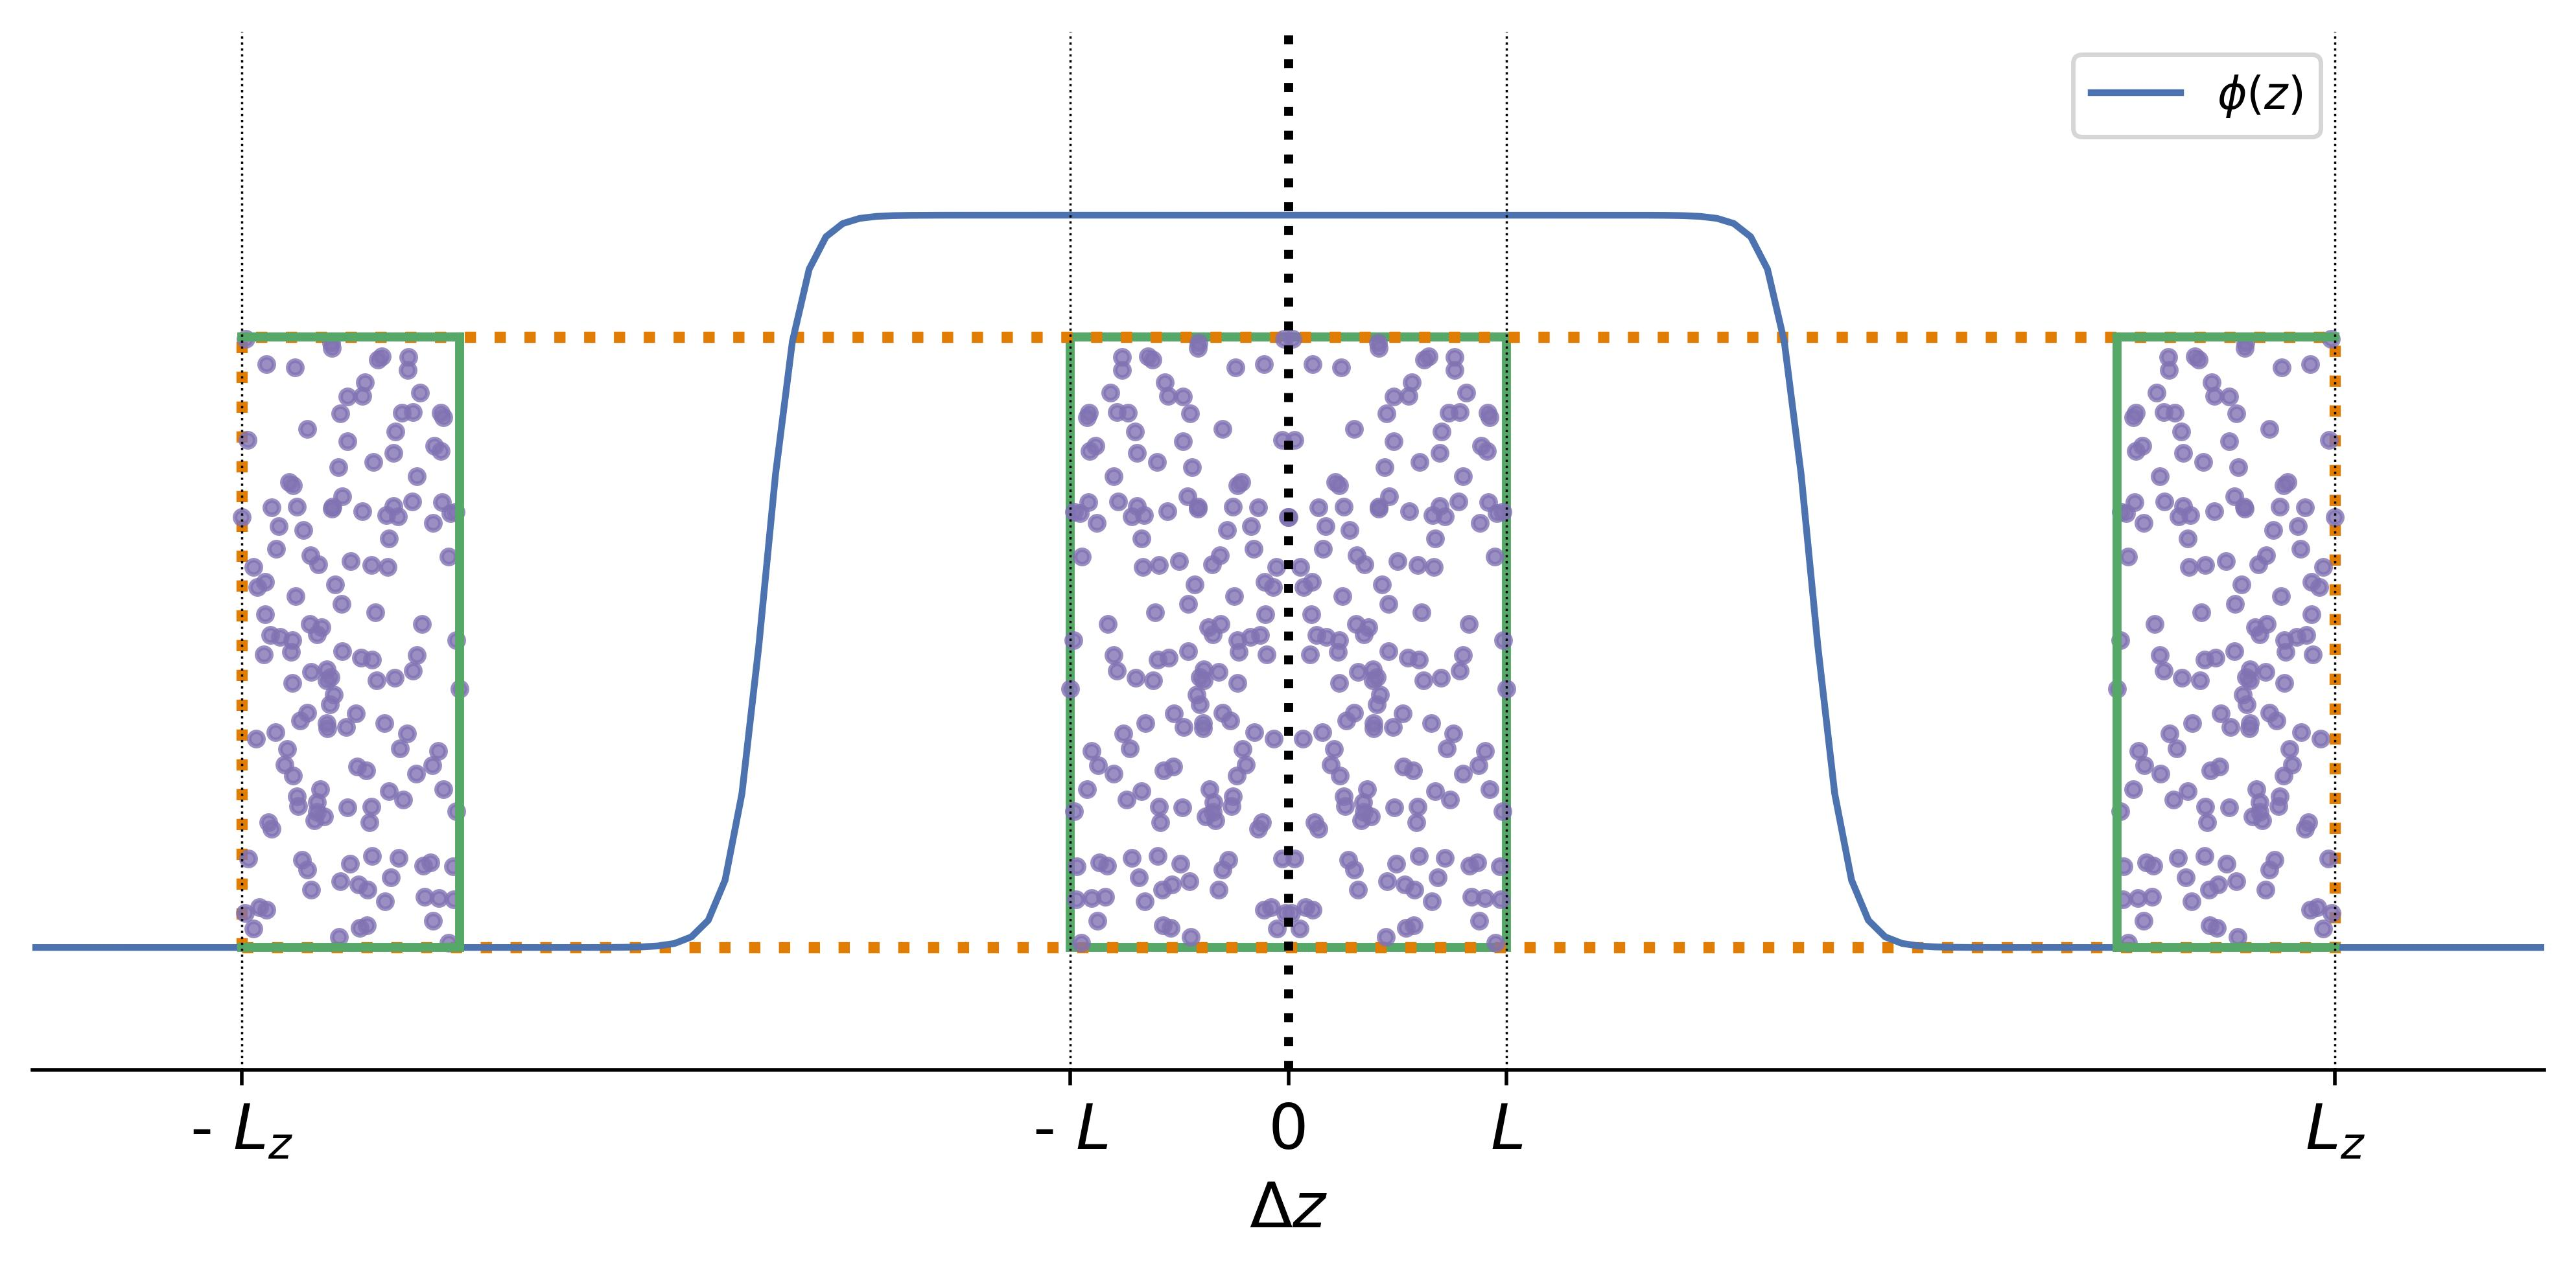
\includegraphics[width=0.65\linewidth]{images/simulationcell.jpg}
    \caption{insert some caption}
    \label{fig:simulation_cell}
\end{figure}

In the $Z$-direction, we introduce a top-hat function $\phi(z)$ in this summation, such that \newline $\phi(z) = 
\begin{cases} 
        1 & \text{if } z \in (-\frac{L_z}{2}, \frac{L_z}{2}) \\
        0 & \text{otherwise}
\end{cases}$
; but to not cause any issues in the function due to its discontinuity, we would be using a smoother version of $\phi(z)$ as follows:
\begin{flalign}
    \phi(z) &= \frac{1}{1+ exp(-\gamma(0.5L_z+z))} + \frac{1}{1+ exp(-\gamma(0.5L_z-z))} -1 \label{eq:1}
\end{flalign}
This function uses a linear combination of two sigmoid functions to make a symmetrical top-hat function about the origin. The constant \textbf{$\gamma$} determines the steepness of the top-hat around the edges. The behaviour of $\phi(z)$ eq.(\ref{eq:1}) is shown in Figure \ref{fig:tophat}.
Other forms of the top-hat functions can also be used; some examples are as follows:
\begin{flalign}
        \phi(z) &= \frac{1}{2}[ \tanh(\gamma(x + 0.5L)) -\tanh(\gamma(x - 0.5L)) ] \\
        \phi(z) &= \frac{2}{\pi}\left[ \arctan \left( e^{\gamma (-x + 0.5L)} \right) + \arctan \left( e^{\gamma (x + 0.5L)} \right) \right]- 1 
\end{flalign}
\begin{figure}[htbp]
    \centering
    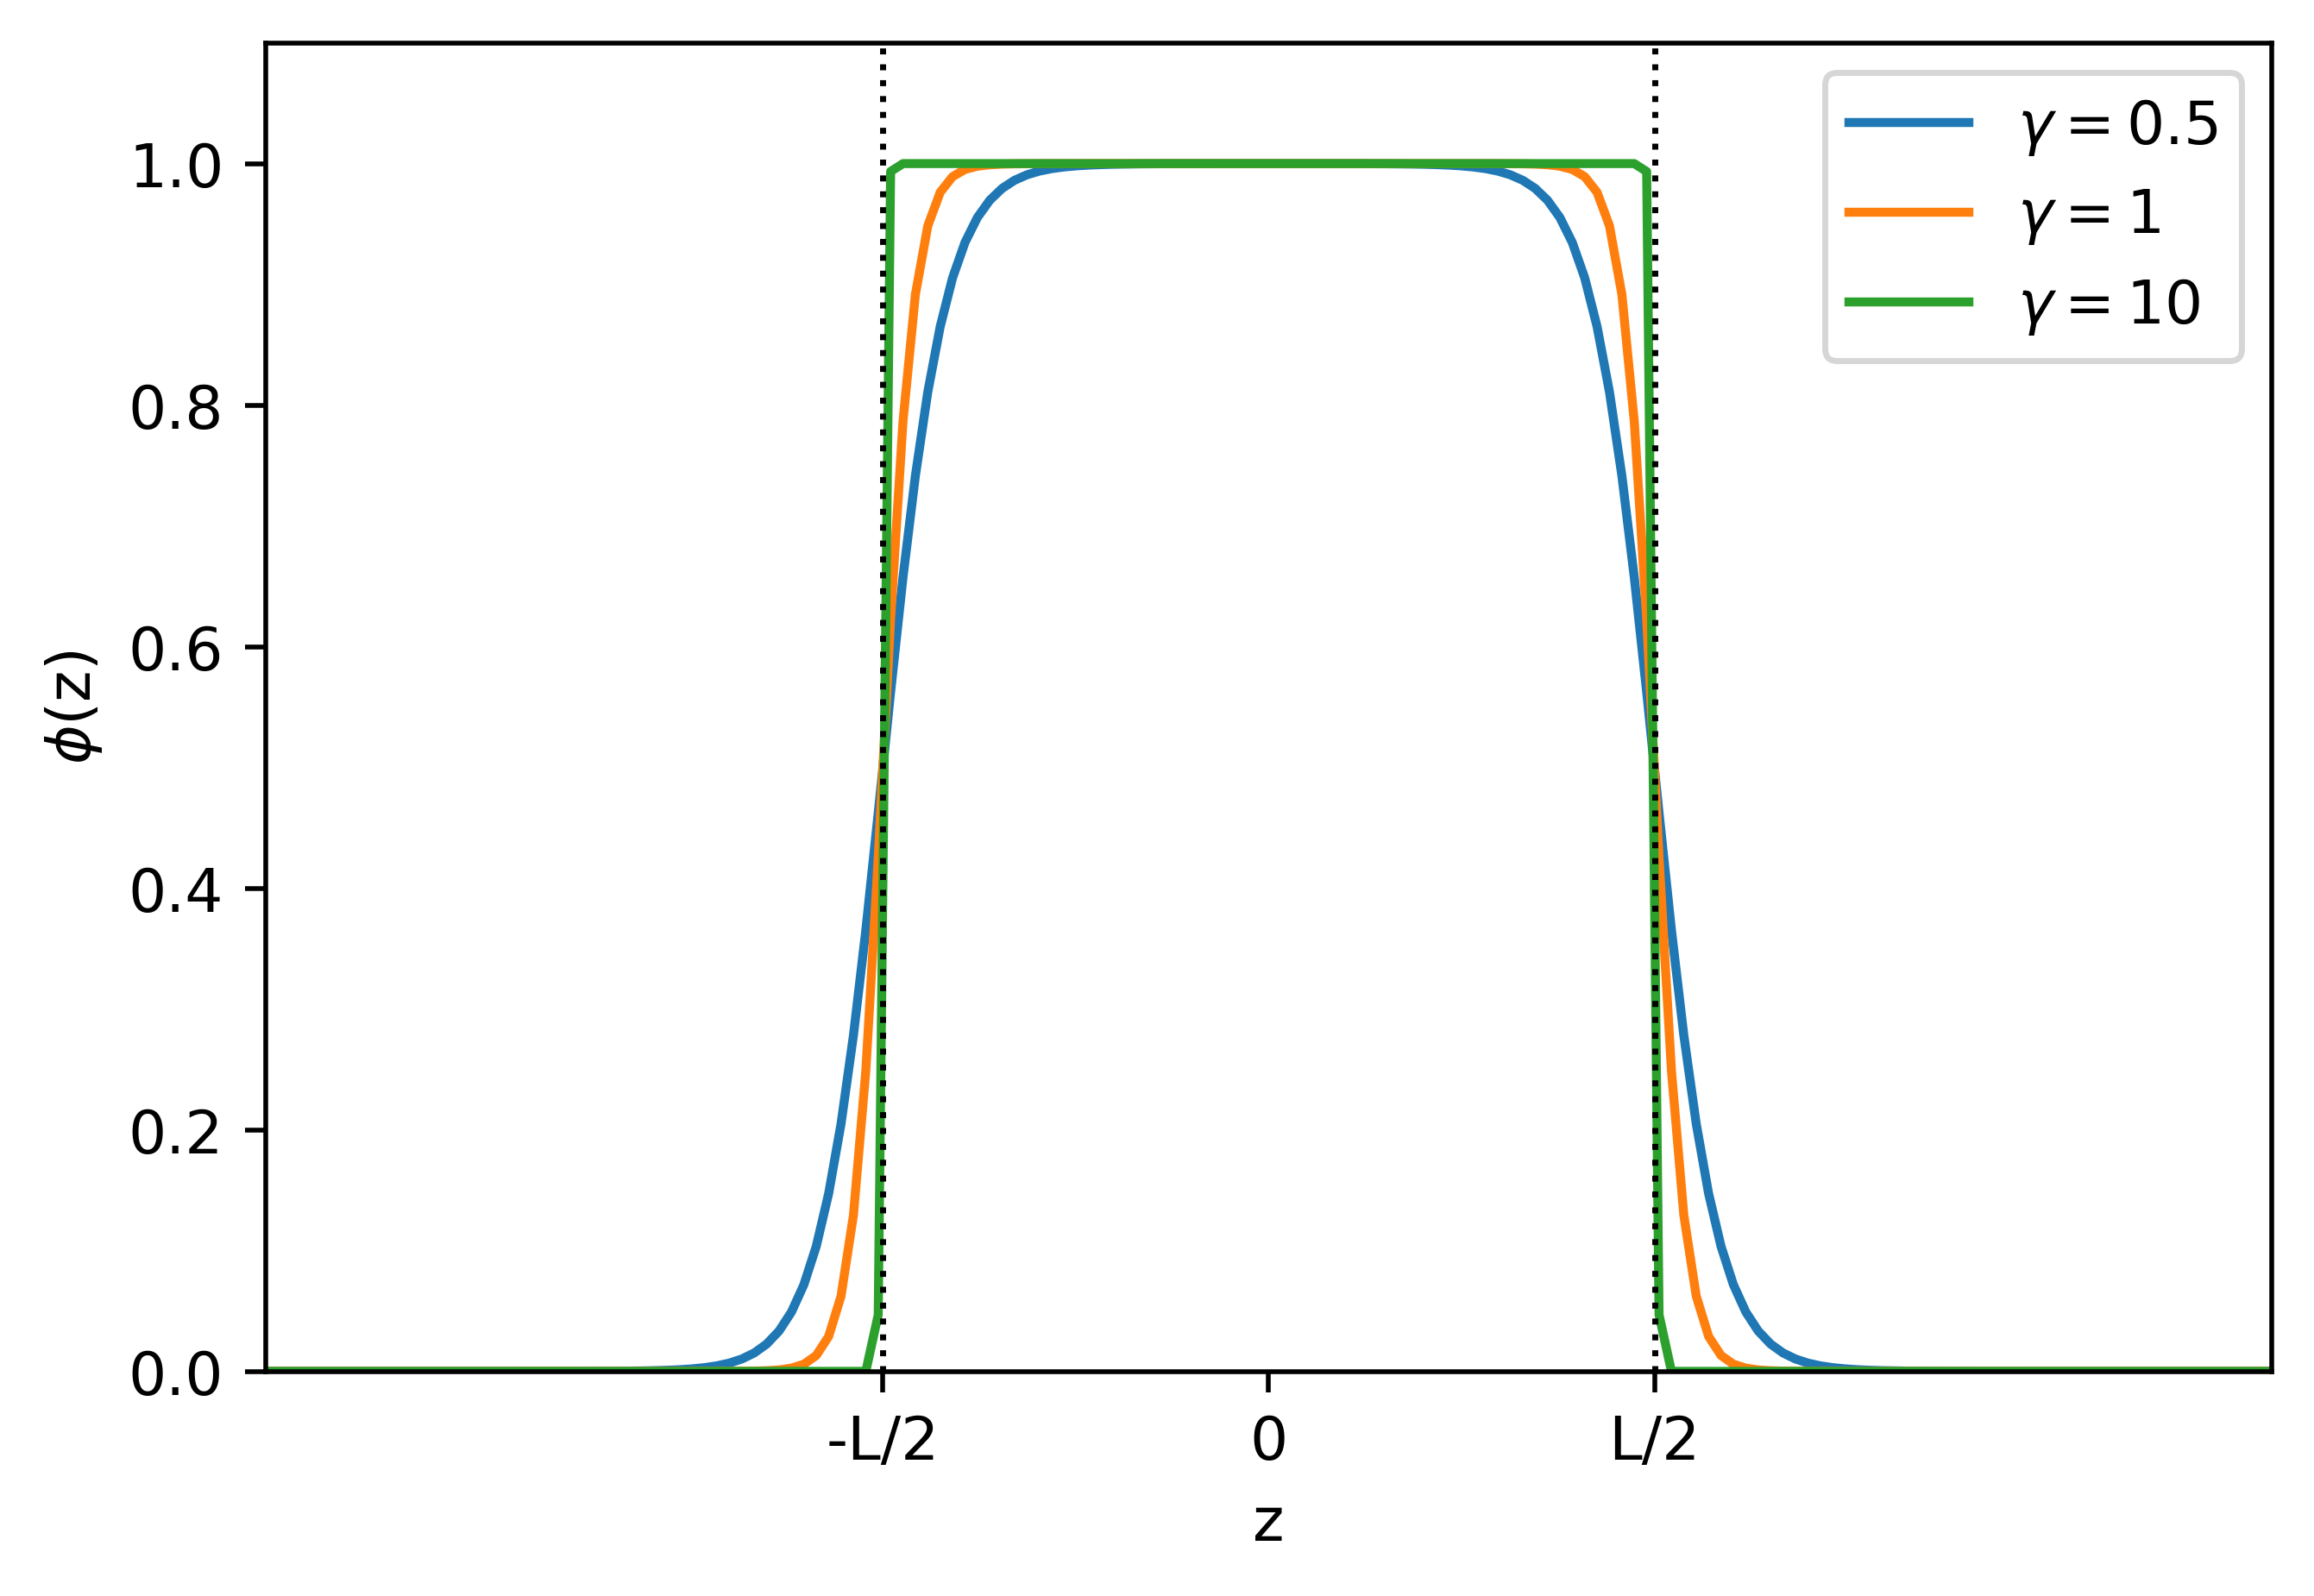
\includegraphics[width=0.5\linewidth]{images/TopHat2.png}
    % \caption{Visualization of Top-hat Function with different $\gamma$. As $\gamma$ increases, the function transitions more sharply at the boundaries, approaching an ideal step function.}
    % \caption{\parbox{0.5\linewidth}{\centering Visualization of Top-hat Function with different $\gamma$. As $\gamma$ increases, the function transitions more sharply at the boundaries, approaching an ideal step function.}}
    \parbox{0.5\linewidth}{\justifying \caption{Visualization of top-hat function for different $\gamma$. As $\gamma$ increases, the function transitions more sharply at the boundaries, approaching an ideal step function.}}
    \label{fig:tophat}
\end{figure}
\subsection{Incorporating the top-hat function}
Since we know that there is no summation of the $M_z$ term in the equation (\ref{eq:main}) in the case of 2D periodic system, which breaks the symmetry in the equation. But our motive is to keep the $M_z$ summation as in the case of 3D periodic system with the help of the top-hat function, whose primary objective is to  count the unwanted contribution of the periodic images in the $z$-direction as zero, as if those images do not exist.

So we insert the $\phi(z)$ function in the reciprocal space summation equation of 3D periodic system, making it behave like 2D periodic system:
\begin{flalign}
    \nonumber(4\pi\epsilon_o)U^{LR} & = \frac{1}{2}\sum_{\vec{M}=-\infty}^{\infty}\sum_{j=1}^{n_p}\sum_{k=1}^{n_p}q_j q_k \frac{{erf}(\alpha|\vec{r_j}-\vec{r_k}+\vec{M}.\vec{L}|)}{|\vec{r_j}-\vec{r_k}+\vec{M}.\vec{L}|} \,\phi(z_{jk}+m_zL_z)  \\
    \nonumber & = \frac{1}{2}\sum_{\vec{M}=-\infty}^{\infty}\sum_{j=1}^{n_p}\sum_{k=1}^{n_p}\frac{2q_j q_k}{\sqrt{\pi}}\int_{0}^{\alpha}dt\,  {exp}(-|\vec{r_j}-\vec{r_k}+\vec{M}.\vec{L}|^2 t^2)\,\phi(z_{jk}+m_zL_z) \\
    \nonumber&=\frac{1}{2}\sum_{\vec{M}=-\infty}^{\infty}\sum_{j=1}^{n_p}\sum_{k=1}^{n_p}\frac{2q_j q_k}{\sqrt{\pi}}\int_{0}^{\alpha}dt\,  {exp}\left[-(x_{jk}+m_xL_x)^2 t^2\right] 
    \times{exp}\left[-(y_{jk}+m_yL_y)^2 t^2\right]\times\\&\hspace{50mm}{exp}\left[-(z_{jk}+m_zL_z)^2 t^2\right] \, \phi(z_{jk}+m_zL_z)
\end{flalign}
We use the Poisson Summation formula to convert this expression from real space to the reciprocal space. \colorbox{yellow}{(see appendix)}
\begin{flalign}
    \nonumber(4\pi\epsilon_o)U^{LR}& =\frac{\sqrt{\pi}}{L_xL_y}\sum_{\vec K=-\infty}^{\infty}\sum_{j=1}^{n_p}\sum_{k=1}^{n_p}q_j q_k \int_{0}^{\alpha}\frac{dt}{t^2}\,{exp}\left(\frac{-\pi^2k_x^2}{L_x^2t^2}+i \frac{2\pi k_xx_{jk}}{L_x}\right)
    \\&\hspace{50mm}
    \times\,{exp}\left(\frac{-\pi^2k_y^2}{L_y^2t^2}+i\frac{2\pi k_yy_{jk}}{L_y}\right)\times C_{k_z}(t)\,{ exp}\left(i\frac{2\pi k_zz_{jk}}{L_z}\right)
\end{flalign}
The term $C_{k_z}(t)$ is expressed as follows:
\begin{flalign*}
     C_{k_z}(t) &=\frac{1}{L_z}\int_{-\infty}^{\infty}ds\hspace{1mm}exp(-i\frac{2\pi n s}{L_z})\hspace{1mm} exp(-s^2t^2)\, \phi(s) 
     % \\ &=\frac{1}{L_z}\int_{-\infty}^{\infty}ds\hspace{1mm}exp(-i\frac{2\pi n s}{L_z})\hspace{1mm} exp(-s^2t^2)\left[\frac{1}{1+ exp(-\gamma(0.5L_z+s))} + \frac{1}{1+ exp(-\gamma(0.5L_z-s))} -1\right]
\end{flalign*}
After a little adjustments
\begin{flalign*}
    \nonumber(4\pi\epsilon_o)U^{LR}& =\frac{\sqrt{\pi}}{L_xL_y}\sum_{\vec K=-\infty}^{\infty}\sum_{j=1}^{n_p}\sum_{k=1}^{n_p}q_j q_k\int_{0}^{\alpha}\frac{dt}{t^2}\,{ exp}\left[i\vec G.(\vec r_j-\vec r_k)\right]\times C_{k_z}(t)\,{ exp}\left(\frac{-1}{4t^2}|\vec G|_{xy}^2\right)\\
    &=\frac{\sqrt{\pi}}{L_xL_y}\sum_{\vec K=-\infty}^{\infty}\left[ \int_{0}^{\alpha}\frac{dt}{t^2}C_{k_z}(t)\,{exp}\left(\frac{-1}{4t^2}|\vec G|_{xy}^2\right)\right]\sum_{j=1}^{n_p}\sum_{k=1}^{n_p}q_j q_k\,{ exp}\left[i\vec G.(\vec r_j-\vec r_k)\right]
\end{flalign*}
Here, $\vec G$ is the reciprocal vector at $(k_x,k_y,k_z)$, expressed as:
\begin{flalign*}
    \vec G &=\frac{k_x2\pi}{L_x}\hat x+\frac{k_y2\pi}{L_y}\hat y+\frac{k_z2\pi}{L_z}\hat z \\
    % \textrm{where $k_x$, $k_y$, $k_z$ $\in$ $\mathbb{Z}^3$}\\
    &=k_xg_x\hat{x}+k_yg_y\hat{y}+k_zg_z\hat{z}
    % \vec{G}&=(\vec{K}.\vec{g}) \qquad\qquad\qquad\qquad  \textrm{here, $\vec{g}$ is the reciprocal vector for $\vec{L}$}
\end{flalign*}
The double summation over indices $j$ and $k$ can be reformulated into a single summation by introducing the structure factor, which is defined as follows:
\begin{flalign*}
    S(\vec G)&=\sum_{j=1}^{n_p}q_j\,exp(i\vec G.\vec r_j)
\end{flalign*}
Therefore, the final expression of the 2D Ewald summation would be
\begin{flalign}
    (4\pi\epsilon_o)U^{LR}& =\frac{\sqrt{\pi}}{L_xL_y}\sum_{\vec K=-\infty}^{\infty}\prime\left[ \int_{0}^{\alpha}\frac{dt}{t^2}C_{k_z}(t)\textrm{ exp}\left(\frac{-1}{4t^2}|\vec G|_{xy}^2\right)\right] |\,S(\vec G)\,|^2
\end{flalign}
Where $\prime$ denotes that the $\vec{K} = 0$ term is not included, it's contribution is 0 if the total charges in the system sums to 0 (electrically neutral system). Here the term inside $[\quad]$ is independent of the \colorbox{yellow}{orientation/distribution} of the system and can be calculated separately before the beginning of the simulation and would not affect overall computational head.

Now we can also use the \colorbox{yellow}{SPME given by essmann et al.} to calculate the stucture factor using the Fast Fourier Transforms.
